\documentclass[10pt,a4paper]{article}
\usepackage[utf8]{inputenc}
\usepackage[spanish, es-tabla]{babel}
\usepackage{amsmath}
\usepackage{amsfonts}
\usepackage{amssymb}
\usepackage{makeidx}
\usepackage{graphicx}
\usepackage{hyperref}
\usepackage{lmodern}
\usepackage{kpfonts}
\usepackage[left=2cm,right=2cm,top=4cm,bottom=2cm]{geometry}
\author{Daniel Vázquez Lago}
\begin{document}
\title{Tensión superficial}
\maketitle \newpage
\tableofcontents \newpage
\section{Objetivos}
El objetivo de esta práctica es determinar la tensión superficial de un líquido, que observaremos en diferentes disoluciones de acetona, en acetona pura y en agua (a temperatura ambiente) así como varía la tensión superficial en función de la temperatura (usando como líquido el agua). De esta forma calcularemos el coeficiente de tensión superficial para cada medida, y su correspondiente incertidumbre.
\section{Introducción teórica}
Se le llama tensión superficial de un líquido a la fuerza que aparece en la superficie de los líquidos debido a las fuerzas intermoleculares, y que nace al introducir un sólido en el. Las moléculas del líquido se ven afectadas por el sólido, y pueden verse atraídas (o no) por las moléculas del sólido. Cuando esto sucede, las moléculas tratarán de mantenerse unidas a dicho sólido, pero como también estarán atraídas por el resto de moléculas, pues se generará una tensión, que aumentará conforme movemos el sólido tratando de despegarlo del líquido. El coeficiente de tensión superficial ($\gamma$)  es una medida de cuanta tensión pueden crear estas moléculas sobre el sólido. \\

De este modo podremos calcularlo solo conociendo la longitud del objeto ($L$) que está en contacto con el agua, la masa del mismo ($m$), que multiplicada por $g$ se convertirá en $P$, el peso, y la fuerza que tenemos que ejercer para arrancarlo ($F'$). En nuestro caso el objeto será un disco. La fórmula que relaciona dichos parámetros es: 
\begin{equation}
F'= 2 \gamma L + P \label{Fuerza de tensión superficial}
\end{equation}
Entonces el coeficiente de regresión lineal será:
\begin{equation}
\gamma = \dfrac{F'-P}{2L} \label{Valor de gamma 1}
\end{equation}
Y teniendo en cuenta que $F=F'-P$ y que $L=\pi d$ (siendo d el diametro del disco):
\begin{equation}
\gamma = \dfrac{F}{2\pi d} \label{Valor de gamma 2}
\end{equation}
Para calcularlo tendremos que tener en cuenta la propagación de incertidumbres, ya que extraeremos su valor usando las medias de $F'$. Por lo tanto usaremos la siguientes fórmula para calcular la media:
\begin{equation}  
\bar{x} = \dfrac{\sum_{i=1}^{n} x_i}{n} \label{media aritmetica}
\end{equation}
Esta para la desviación típica:
\begin{equation}
s_A(x)=\sqrt{\dfrac{\sum_{i=1}^n (x_i-\bar{x})^2}{n-1}} \label{desviación típica de los datos en una media}
\end{equation}
Y la desviación típica de la media (que es realmente la que nos interesa ya que a partir de esta calcularemos la desviación típica de $\gamma$:
\begin{equation}
s_A(\bar{x})=\dfrac{s_A(x)}{\sqrt{n}} \label{Desviación estandar de la media}
\end{equation}
Y teniendo en cuenta la incertidumbre de tipo B (	que es la incertidumbre de medida directa, afectada por el aparato y otros factores) que se calcularía, en nuestro caso, con la precisión de la medida. Así realidad la incertidumbre de la media sería bastante mayor, y combinando ambas:
\begin{equation}
s_C(x) = \sqrt{[s_A(\bar{x}]^2+[s_B(x)]^2} \label{incertidumbre combinada}
\end{equation}
Ahora podríamos calcular la incertidumbre de $\gamma$ y $F$ usando la siguiente fórmula:
\begin{equation}
s(y)=\sqrt{\sum_i (\dfrac{\partial y}{\partial x_i})^2s^2(x_i)} \label{propagación de inciertidumbres}
\end{equation}

Entonces las fórmulas de las incertidumbres:
\begin{equation}
s(F)=\sqrt{s^2(F')+s^2(P)}
\label{inceridumbre F}
\end{equation}
\begin{equation}
s(\gamma)=\sqrt{(\dfrac{1}{2 \pi d})^2s^2(F)+(-\dfrac{F}{2\pi d^2})^2s^2(d)}
\label{incertidumbre gamma}
\end{equation}
Ahora si podríamos calcular el coeficiente de tensión superficial tanto para el agua como para las diferentes disoluciones de acetona (y su incertidumbre). Sin embargo la segunda parte de la práctica nos pide calcular este valor en función de la temperatura, que viene dado por una regresión lineal de tal forma que: 
\begin{equation}
\gamma=a - bT \label{regresion lineal}
\end{equation}
Entonces tendremos que usar todas las fórmulas aplicadas a las regresiones lineales, aunque para facilitar la lectura de la práctica no escribirimos todas estas fórmulas, simplemente usaremos programas informáticos para calcular estos valores y sus incertidumbres. Además contaremos con una gráfica donde se podrán visualizar los cálculos.
\subsection{Montaje experimental y procedimiento de medida}
\section{Análisis de datos}
En la siguiente tabla representamos ciertas medidas que serán usadas a lo larga de toda la práctica:

\begin{table}[h]
\begin{center}
\begin{tabular}{|c|c|c|c|} \hline
$P  \ (N)$ & $s(P) \ (N)$ & $d \ (m)$ & $s(d) \ (m)$ 
  \\ \hline
0,069  & 0,001 & 0,063  & 0,002 
  \\  \hline
\end{tabular}
\caption{valores del peso y de el diámetro del disco con su incertidumbre}
\label{tab:masa y peso}
\end{center}
\end{table}

\subsection{Estudio de la tensión superficial a temperatura ambiente}

\begin{table}[h]
\begin{center}
\begin{tabular}{|c|c|c|}
\hline
medida (i) & $F' \ (N) $ & $s(F') \ (N) $ 
  \\  \hline
1 & 0,100 & 0,001 
  \\ 
2 & 0,099  & 0,001 
  \\ 
3 & 0,0995  & 0,001 
  \\ 
4 & 0,100 & 0,001  
  \\ 
5 & 0,100 & 0,001  
  \\ 
6 & 0,100 & 0,001 
  \\ 
7 & 0,0998 & 0,001  
  \\ 
8 & 0,100 & 0,001  
  \\ 
9 & 0,100 & 0,001 
  \\ 
10 & 0,101 & 0,001  
  \\ \hline
\end{tabular}
\caption{valores de $F'$ para el agua a temperatura ambiente (aproximadamente 22º)}
\end{center}
\label{tab:F'  }
\end{table}

Antes de continuar vamos a explicar un factor que puede llamar la atención. Existen ciertos valores que poseen mas cifras significativas que las que tiene la incertidumbre (que es la precisión del aparato). Esto se debe a la baja precisión del aparato, con un alcance mucho menos preciso que la propia vista humana. Por lo tanto, aunque realmente los valores deberían ser de 0,1, cogimos esos valores porque se adecuaban más, al estar entre 0,1 y 0,999. Dicho esto: son valores tomados de manera subjetiva, pero más precisa. De todos modos no implica ningún cambio en la incertidumbre de los propios datos. \\

Ahora usando tanto la ecuación \ref{media aritmetica} y \ref{incertidumbre combinada} podremos hallar el valor medio de $F'$ y la incertidumbre. De esta forma tenemos que:
$$ \bar{F'}=0,09993, \ \ s(F')=0,00050, \ \ s(\bar{F'})=0,00017, \ \ s_C(\bar{F'})=0,001 $$

\begin{table}[h!] %valores f'
\begin{center}
\begin{tabular}{|c|c|}
\hline
$F' \ (N)$ &  $s(F') \ (N)$ \\ \hline
0,09993 & 0,001 \\ \hline
\end{tabular}
\caption{Valores finales de F' y su incertidumbre}

\label{tab:valores finales F' a temperatura ambiente}
\end{center}
\end{table}

\begin{flushleft}
Ahora a partir de los datos tomados en la Tabla \ref{tab:masa y peso} y \ref{tab:valores finales F' a temperatura ambiente} tenemos que: 
\end{flushleft}

$$ F = 0,09993 - 0,069 = 0,03093 \ N$$
Y que su incertidumbre es:
$$ s(F)=\sqrt{0,001^2+001^2}=0,014$$
Por lo que en total tenemos que:

\begin{table}[h!] %tabla f
\begin{center}
\begin{tabular}{|c|c|}
\hline
$F \ (N)$ &  $s(F) \ (N)$ \\ \hline
0,0309 & 0,0014 \\ \hline
\end{tabular}
\caption{Valores finales de F y su incertidumbre}
\label{tab:valores finales F a temperatura ambiente}
\end{center}
\end{table} 

Y teniendo ya en cuenta todo esto ya somos capaces de calcular $\gamma$: 
$$ \gamma = \dfrac{0,031}{2 \pi 0,063} = 0,0781; \ \ \ s(\gamma)=0,0025$$
Por lo tanto acabaríamos la primera parte de la práctica: determinar el coeficiente tensión superficial del agua a temperatura ambiente. Representándolo en una tabla para que quede mejor expuesto:

\begin{table}[h!] %tabla gamma
\begin{center}
\begin{tabular}{|c|c|}
\hline
$\gamma  \ (N/m)$ &  $s(\gamma) \ (N/m)$ \\ \hline
0,0781 & 0,0025 \\ \hline
\end{tabular}
\caption{Valores finales de $\gamma$ y su incertidumbre}

\label{tab:valores finales F a temperatura ambiente}
\end{center}
\end{table} 

\subsection{Estudio de la tensión superficial a diferentes temperaturas}
Ahora estudiaremos el comportamiento del coeficiente de tensión superficial en función de la temperatura del agua, teniendo en cuenta que $\gamma = a + bT$. La tabla \ref{tab:t vs f'} muestra los valores de $\gamma$ en función de $T$  y la propia temperatura. Entonces:
$$ b=-0,004857;\ \ s(b)= 0,000022;\ \ a=0.0872;\ \ s(a)=	0,0012;\ \ r=0,95 $$
Tal y como se puede ver el coeficiente de regresión lineal no es muy bueno, pero es evidente que va a ser así ya que la precisión de los aparatos no es muy buena, al igual que el momento de ruptura de la película de agua es realmente complicado de medir de manera exacta. Esto  se ve muy bien en la representación gráfica de la figura \ref{fig:plot1}, donde se puede ver como los puntos están bastante separados de la regresión lineal. De todas maneras nos sirve como aproximación, y demuestra se cumple la relación lineal entre el coeficiente de tensión superficial de un líquido y su temperatura.
\begin{table}[h] %tabla de las temperaturas
\begin{center}
\begin{tabular}{|c|c|c|c|c|c|c|}
\hline 
medida & $T$ (Cº) & s($T$) (Cº) & $F' \ (N)$ & $ s(F') \ (N) $ & $\gamma \ (N/m)$ & $s(\gamma) \ (N/m)$
  	\\  \hline
1 & 	 83,1 & 	 0,1 & 	 0,088 & 	 0,001 & 	 0,0480 & 	 0,0025
  	\\ 
2 & 	 81,1 & 	 0,1 & 	 0,089 & 	 0,001 & 	 0,0505 & 	 0,0025
  	\\ 
3 & 	 79,3 & 	 0,1 & 	 0,0895 & 	 0,001 & 	 0,0518 & 	 0,0025
  	\\ 
4 & 	 78,8 & 	 0,1 & 	 0,089 & 	 0,001 & 	 0,0505 & 	 0,0025
  	\\ 
5 & 	 75,6 & 	 0,1 & 	 0,090 & 	 0,001 & 	 0,0531 & 	 0,0025
  	\\ 
6 & 	 75,4 & 	 0,1 & 	 0,089 & 	 0,001 & 	 0,0505 & 	 0,0025
  	\\ 
7 & 	 72,0 & 	 0,1 & 	 0,090 & 	 0,001 & 	 0,0531 & 	 0,0025
  	\\ 
8 & 	 71,8 & 	 0,1 & 	 0,090 & 	 0,001 & 	 0,0531 & 	 0,0025
  	\\ 
9 & 	 66,9 & 	 0,1 & 	 0,090 & 	 0,001 & 	 0,0531 & 	 0,0025
  	\\ 
10 & 	 65,6 & 	 0,1 & 	 0,091 & 	 0,001 & 	 0,0556 & 	 0,0025
  	\\ 
11 & 	 60,2 & 	 0,1 & 	 0,091 & 	 0,001 & 	 0,0556 & 	 0,0025
  	\\ 
12 & 	 60,0 & 	 0,1 & 	 0,091 & 	 0,001 & 	 0,0556 & 	 0,0025
  	\\ 
13 & 	 53,2 & 	 0,1 & 	 0,092 & 	 0,001 & 	 0,0581 & 	 0,0025
  	\\ 
14 & 	 47,1 & 	 0,1 & 	 0,093 & 	 0,001 & 	 0,0606 & 	 0,0025
  	\\ 
15 & 	 41,9 & 	 0,1 & 	 0,094 & 	 0,001 & 	 0,0632 & 	 0,0025
  	\\ 
16 & 	 40,7 & 	 0,1 & 	 0,094 & 	 0,001 & 	 0,0632 & 	 0,0025
  	\\ 
17 & 	 36,3 & 	 0,1 & 	 0,096 & 	 0,001 & 	 0,0682 & 	 0,0025
  	\\ 
18 & 	 30,5 & 	 0,1 & 	 0,096 & 	 0,001 & 	 0,0682 & 	 0,0025
  	\\ 
19 & 	 27,5 & 	 0,1 & 	 0,098 & 	 0,001 & 	 0,0733 & 	 0,0025
  	\\ 
20 & 	 24,6 & 	 0,1 & 	 0,100 & 	 0,001 & 	 0,0783 & 	 0,0025
  	\\ 
21 & 	 18,9 & 	 0,1 & 	 0,101 & 	 0,001 & 	 0,0808 & 	 0,0025
  	\\ 
22 & 	 18,8 & 	 0,1 & 	 0,100 & 	 0,001 & 	 0,0783 & 	 0,0025
  	\\ 
23 & 	 15,5 & 	 0,1 & 	 0,102 & 	 0,001 & 	 0,0834 & 	 0,0025
  	\\ 
24 & 	 13,1 & 	 0,1 & 	 0,102 & 	 0,001 & 	 0,0834 & 	 0,0025
  	\\ 
25 & 	 11,9 & 	 0,1 & 	 0,102 & 	 0,001 & 	 0,0834 & 	 0,0025
  	\\  \hline
\end{tabular}
\caption{valores de $F'$ con diferentes temperaturas en el agua}
\label{tab:t vs f'}
\end{center}
\end{table}

\begin{figure}[h!]
\centering
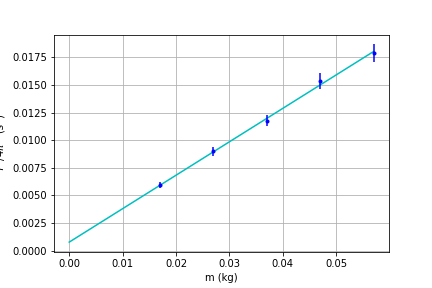
\includegraphics[width=11cm, height=7cm]{plot1.png}
\caption{Representación de $\gamma$ frente a la temperatura del agua}
\label{fig:plot1}
\end{figure}

\newpage

\subsection{Estudio de la tensión superficial con diferentes disoluciones de acetona}
Como podemos ver en la tabla \ref{tab:F' vs acetona} tenemos que el coeficiente de tensión superficial se reduce a medida que aumentamos la concentración de acetona: al principio de una manera muy rápida, y a medida que este porcentaje es mucho mas alto se va reduciendo lo que aumenta. \\

De esto podemos extraer una conclusión: que no tiene un comportamiento lineal, es decir, no se reduce de manera constante dicho coeficiente. ¿A que se puede deber esto? Pues bien, al mezclar dos líquidos aquel con menor $\gamma$ se sitúa en la superficie,  por lo que aunque su concentración sea de un 10\%, en la superficie habrá una mayor concentración de el, en nuestro caso de acetona. Eso explica porque baja de manera drástica al principio, y porque ya cuando hay mucha concentración no baja tanto. Esto se debería a que cuando el porcentaje es muy alto, realmente la cantidad de acetona en la superficie no esta cambiando prácticamente, que es lo que realmente influye en $\gamma$. \\

Este cambio se puede observar muy bien en la figura \ref{fig:plot2}, en la cual la linea azul es una aproximación por una parábola (polinomio de orden dos).
\begin{table}[h] %tabla de las disoluciones
\begin{center}
\begin{tabular}{|c|c|c|c|c|c|c|}
\hline
i & 	 \% acetona & 	 $F' \ (N)$ & 	 $s(F') \ (N)$ & 	 $\gamma \ (N/m) $ & 	 $s(\gamma) \ (N/m) $ \\  \hline
1 & 	 10 & 	 0,092 & 	 0,001 & 	 0,0581 & 	 0,0025 \\ 
2 & 	 20 & 	 0,088 & 	 0,001 & 	 0,0480 & 	 0,0025 \\ 
3 & 	 30 & 	 0,086 & 	 0,001 & 	 0,0429 & 	 0,0025 \\ 
4 & 	 40 & 	 0,084 & 	 0,001 & 	 0,0379 & 	 0,0025 \\ 
5 & 	 50 & 	 0,082 & 	 0,001 & 	 0,0328 & 	 0,0025 \\ 
6 & 	 60 & 	 0,082 & 	 0,001 & 	 0,0328 & 	 0,0025 \\ 
7 & 	 70 & 	 0,081 & 	 0,001 & 	 0,0303 & 	 0,0025 \\ 
8 & 	 80 & 	 0,080 & 	 0,001 & 	 0,0278 & 	 0,0025 \\ 
9 & 	 90 & 	 0,080 & 	 0,001 & 	 0,0278 & 	 0,0025 \\ 
10 & 	 100 & 	 0,079 & 	 0,001 & 	 0,0253 & 	 0,0025 \\ 
\hline

\end{tabular}
\caption{valores de $\gamma$ para diferentes disoluciones de acetona}

\label{tab:F' vs acetona}
\end{center}
\end{table}

\begin{figure}[h]
\centering
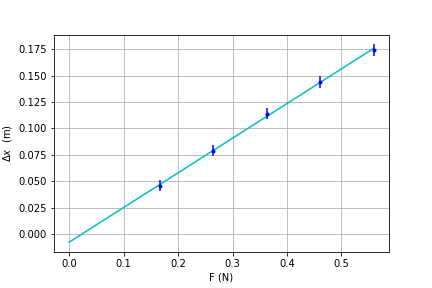
\includegraphics[width=11cm, height=7cm]{plot2.png}
\caption{Representación de $\gamma$ frente al porcentaje de acetona en la disolución}
\label{fig:plot2}
\end{figure}
\subsection{Conclusión}
\subsection{Bibliografía}
\end{document}
